%
%  A presentation of ZMailer for  FUUG at SEA 2000 conference
%
%     FUUG = Finnish Unix User Group
%     SEA  = The baltic sea; cruising from Helsinki to Stockholm, and back
%
%  Matti Aarnio, 12-Sep-2000
%

\documentclass[a4paper,landscape]{slides}

\setlength{\topmargin}{-40pt}
\setlength{\headsep}{2EM}
\setlength{\footskip}{3\footskip}

\usepackage[dvips]{color}
\usepackage[dvips]{epsfig}
\usepackage{float}
\usepackage{wrapfig}
\usepackage{verbatim}

\setlength{\wrapoverhang}{0.3in}

\newcommand{\SLIDEFOOT}{\centerline{\rm Matti Aarnio $<matti.aarnio@sonera.fi>$}}
\newcommand{\SLIDEHEAD}{\centerline{\tiny\rm FUUG @ SEA-2000:   ZMailer}}

\newcommand{\ZM}{ZMailer}

\begin{document}
\pagestyle{plain}

%%%%%%%%%%%%%%%%%%%%%%%%%%%%%%%%%%%%%%%%%%%%%%%%%%%%%%%%%%%%%%%%%

\begin{slide}

\begin{center}
 ZMailer --- A Different Kind of MTA
\end{center}

\vfill

\begin{center}
 
\epsfig{file=zmailer-logo.ps}
\end{center}

\vfill

\end{slide}

%%%%%%%%%%%%%%%%%%%%%%%%%%%%%%%%%%%%%%%%%%%%%%%%%%%%%%%%%%%%%%%%%

\begin{overlay}

\begin{center}
 ZMailer --- A Different Kind of MTA
\end{center}

\vfill

  A presentation of ZMailer for  FUUG at SEA 2000 conference

     FUUG = Finnish Unix User Group

     SEA  = The baltic sea; cruising from Helsinki to Stockholm, and back

 Matti Aarnio, 12-Sep-2000

The overlays and notes are supplementaty material, which supports
the mainline slides.

\end{overlay}

%%%%%%%%%%%%%%%%%%%%%%%%%%%%%%%%%%%%%%%%%%%%%%%%%%%%%%%%%%%%%%%%%


\begin{slide}
\centerline{\large A bit of History}

\vfill
\ZM{} was created at {\it University of Toronto} around 1986 by
Mr. {\it Rayan Zachariassen} (hence the ``Z'' in the name.)

Rayan went to private sector around 1992, and $ZMailer$ development
was essentially abandoned by him.

Since then, yours truly has been hacking at it developing all kinds
of extensions for modern Internet email.

\vfill

\end{slide}

%%%%%%%%%%%%%%%%%%%%%%%%%%%%%%%%%%%%%%%%%%%%%%%%%%%%%%%%%%%%%%%%%


\begin{slide}

\centerline{\large \ZM{} structure}

\begin{wrapfigure}[11]{l}{3in}
 \epsfig{file=zmprocs.ps,width=2.7in}
\end{wrapfigure}

\ZM{} consists of several main subsystems running in coordinated,
although separate existence.  This means also that any of the subsystems
can be shut down for a while without harming other subsystem functionality.

The task-transfer in between the subsystems is done via
the filesystem -- {``\it spool''}.
Performance of this filesystem is usually the ultimate system thoughput limit.

\vfill
\centerline{\it There are no suid-anything programs in this system!}

\vfill

\end{slide}

%%%%%%%%%%%%%%%%%%%%%%%%%%%%%%%%%%%%%%%%%%%%%%%%%%%%%%%%%%%%%%%%%


\begin{slide}

\centerline{\large \ZM{} structure}

\begin{wrapfigure}[6]{l}{3in}
 \epsfig{file=zmprocs.ps,width=2.7in}
\end{wrapfigure}

Input subsystems: {\it sendmail, smtpserver, rmail, mail(3)} library

Routing subsystem: {\it router}

Delivery subsystem: {\it scheduler,} and {\it transport agents}

Plus a set of administrative tools.

The goal has been that each subsystem uses minimal possible amount of
resources, and privileges to achieve its task.

There are also resource usage limitation
features built in.
\vfill

\end{slide}

%%%%%%%%%%%%%%%%%%%%%%%%%%%%%%%%%%%%%%%%%%%%%%%%%%%%%%%%%%%%%%%%%


\begin{slide}

\centerline{\large \ZM{} subsystems: {\it ``POSTOFFICE/''}}

The \verb!$POSTOFFICE/! is \ZM{}'s way of referring to filesystem
where a few basic things are guaranteed to happen:
\begin{enumerate}
\item moving files around with {\it rename(2)} and/or {\it link(2),} and
      {\it unlink(2)} works just fine in between different directories
\item i-node numbers are preserved over {\it rename(2)}, and {\it link(2)}
	system calls
\end{enumerate}

There are filesystems where these two things don't happen, e.g. possibly
{\it link(2)} can't be done in between directories.  Such ones are not
suitable for \ZM's \verb!$POSTOFFICE/! partition use.

\end{slide}

%%%%%%%%%%%%%%%%%%%%%%%%%%%%%%%%%%%%%%%%%%%%%%%%%%%%%%%%%%%%%%%%%


\begin{slide}

\centerline{\large \ZM{} subsystems: {\it ``sendmail''}}

For normal local system use there needs to be a well-known
submission interface for email.  A de-facto one is {\it sendmail.}

\ZM's {\it sendmail} implements most of message submission options
of the real {\it sendmail(8).}

Many of {\it sendmail(8)} options are meaningless in \ZM{}, and thus
they are ignored, or in case of several administrative functions,
start subsystems in interactive test mode and/or just plain complain
loudly.

For message submission, \ZM's {\it sendmail} is extremely
{\it lightweight} one.  Just writing the message envelope and
message to the file, and moving it to {\it router} subsystem's care.


\vfill

\end{slide}

\begin{slide}

\centerline{\large \ZM{} subsystems: {\it ``sendmail''}}

In normal message submission the {\it sendmail} will just spool
the message into \verb!$POSTOFFICE/router/!, however if option
{\it ``-v''} is used, process is left behind to poll a message
specific ``verbose trace'' log file, and its content is copied
to STDERR of the process.

The verbose trace copy process ends when the {\it scheduler}
process writes a line:
\begin{verbatim}
  scheduler done ....
\end{verbatim}
to the log file.

\ZM's {\it sendmail} is just message submission interface, like
also the {\it smtpserver}, and  {\it libzmailer.a}  contained
{\it mail(3).}

\vfill

\end{slide}

%%%%%%%%%%%%%%%%%%%%%%%%%%%%%%%%%%%%%%%%%%%%%%%%%%%%%%%%%%%%%%%%%


\begin{slide}

\centerline{\large \ZM{} subsystems: {\it ``smtpserver''}}

\begin{wrapfigure}[12]{l}{5.15in}
\tiny
\begin{tabular}{ll}
ESMTP RFC's \\

1425/1651/2045 & EHLO framework \\
1426/1652 & 8BITMIME \\
1427/1653/1870 & SIZE \\
1830 & CHUNKING \\
1854/2197 & PIPELINING \\
1891 & DSN \\
1985 & ETRN \\
2034 & ENHANCEDSTATUSCODES \\
2487 & STARTTLS \\
2554+MS & AUTH LOGIN \\
2554+Netscape & AUTH=LOGIN
\end{tabular}
\end{wrapfigure}
\ZM's {\it smtpserver} subsystem implements a rich set of enhanced SMTP
features defined over the last 10 or so years.

At the same time it aims to be lightweight, fast protocol receiver with
ability to quickly verify incoming protocol stream syntax conformance,
but it can also be configured to behave sloppily in this regard.

\vfill

\end{slide}

\begin{slide}

\centerline{\large \ZM{} subsystems: {\it ``smtpserver''}}

The {\it smtpserver} can do interactive routing analysis of
{\it MAIL FROM:} and {\it RCPT TO:} phase envelope addresses
by running a router process synchronously underneath itself,
however that is seriously heavy-weight thing, and really taxes
system performance for no practically usefull thing.

A more usefull approach is simply to do SMTP MX/A routing rules
analysis of source and destination envelope addresses, with
some control rules from a few local database files giving the
system an idea of which domains are local, and which are rules
for finding which domains are our customers.

There are also some experimental hooks to run external message
content analysis 

\vfill

\end{slide}

%%%%%%%%%%%%%%%%%%%%%%%%%%%%%%%%%%%%%%%%%%%%%%%%%%%%%%%%%%%%%%%%%


\begin{overlay}
\small
\centerline{{\it ``smtpserver.conf''}}
\tiny

\begin{verbatim}
#
# smtpserver.conf - autogenerated edition
#
#PARAM maxsize              10000000    # Same as -M -option
#PARAM min-availspace           5000    # Minimum free in POSTOFFICE after
#                                       # message has arrived; in KILOBYTES.
#PARAM max-error-recipients        3    # More than this is propably SPAM!
#PARAM MaxSameIpSource            10    # Max simultaneous connections
#                                       # from any IP source address
#PARAM MaxParallelConnections    800    # Max simultaneous connections
#                                       # in total to the server
#PARAM TcpRcvBufferSize        32000    # Should not need to set!
#PARAM TcpXmitBufferSize       32000    # Should not need to set!
#
#PARAM ListenQueueSize            10    # listen(2) parameter
#
#PARAM RcptLimitCount          10000    # Max number of recipients for one
#                                       # MAIL FROM session. Minimum: 100
#
#PARAM use-tcp-wrapper                  # Use tcp-wrapper in addition to
#                                       # actual input policy controls.
\end{verbatim}
\end{overlay}
\begin{overlay}
\small
\centerline{{\it ``smtpserver.conf''}}
\tiny
\begin{verbatim}
#PARAM BindPort                   25    # Binding port
#PARAM BindAddress         [0.0.0.0]    # Binding address - for multihomers..
#PARAM BindAddress       [IPv6.0::0]    # and here is for IPv6 - NO SPACES!
#
# Enables of some commands:
PARAM   DEBUGcmd
PARAM   EXPNcmd
PARAM   VRFYcmd
PARAM   enable-router   # This is a security decission for you.
#                       # This is needed for EXPN/VRFY and interactive
#                       # processing of MAIL FROM and RCPT TO addresses.
#                       # However it also may allow external user entrance
#                       # to ZMailer router shell environment with suitably
#                       # pervert input, if quotation rules are broken in
#                       # the scripts.
\end{verbatim}
\end{overlay}
\begin{overlay}
\small
\centerline{{\it ``smtpserver.conf''}}
\tiny
\begin{verbatim}
PARAM   smtp-auth       # enable if you want to allow SMTP to autenticate
#                       # with the default code against system  /etc/passwd
#                       # (or whatever source  getpwnam() uses for it..)
#
PARAM  AUTH-LOGIN-also-without-TLS
#                       # Enable, if the "AUTH LOGIN" is to be allowed to
#                       # be used without running under SSL/TLS security
#                       # envelope.
#
#PARAM  MSA-mode        # Message Submission Agent mode. Require
#                       # successful user authentication during SMTP
#                       # sessions initiated from outside of the trusted
#                       # networks or the networks with relaying enabled
#                       # (see "fulltrustnet" and "relaycustnet" in
#                       # smtp-policy.src file).
#
PARAM   deliverby 60
#                       # RFC 2852 defined deliverby machinery.
\end{verbatim}
\end{overlay}
\begin{overlay}
\small
\centerline{{\it ``smtpserver.conf''}}
\tiny
\begin{verbatim}
#PARAM  SMTP-auth-pipe /path/to/program
#                       # External authentication program. The
#                       # authenticator should read a username from
#                       # command line and a password from standard input.
#                       # Exit status 0 means successful authentication.
#
# Disablers of some facility adverticements
#PARAM  NoEHLO
#PARAM  NoPIPELINING
#PARAM  No8BITMIME
PARAM   NoCHUNKING
#PARAM  NoDSN
#PARAM  NoETRN
PARAM  no-multiline-replies # except to EHLO (Bloody M$ RFC821/AppE violators)
\end{verbatim}
\end{overlay}
\begin{overlay}
\small
\centerline{{\it ``smtpserver.conf''}}
\tiny
\begin{verbatim}
# HDR220 metatags:
#  %% -- '%' character
#  %H -- SS->myhostname
#  %I -- '+IDENT' if 'identflg' is set
#  %V -- VersionNumb
#  %T -- curtime string
#  %X -- xlatelang parameter
#
#PARAM hdr220 %H ZMailer ESMTP-server %V running at Yoyodyne Propulsion Inc
#PARAM hdr220 %H ESMTP (NO UCE)(NO UBE) our local time is now %T
#
# Note above the "ESMTP" words are present because *some* MTA systems won't
# do EHLO greeting, unless they see "ESMTP" - against RFC 1869 part 4.
# "EHLO is to be done blindly, server responses are not to be studied for
#  any possible 'ESMTP' keyword!"
\end{verbatim}
\end{overlay}
\begin{overlay}
\small
\centerline{{\it ``smtpserver.conf''}}
\tiny
\begin{verbatim}
PARAM help -------------------------------------------------------------
PARAM help  This mail-server is at Yoyodyne Propulsion Inc.
PARAM help  Our telephone number is: +1-234-567-8900, and
PARAM help  telefax number is: +1-234-567-8999
PARAM help  Our business-hours are Mon-Fri: 0800-1700 (Timezone: -0700)
PARAM help
PARAM help  Questions regarding our email service should be sent via
PARAM help  email to address  <postmaster@OURDOMAIN>
PARAM help  Reports about abuse are to be sent to: <abuse@OURDOMAIN>
PARAM help -------------------------------------------------------------
#
# Uncomment following for not to strip incoming addresses of format:
# <@aa,@bb:cc@dd> into non-source-routed base form: <cc@dd>
#
#PARAM  allowsourceroute # DON'T ENABLE UNLESS YOU USE ROUTER BASED
#                        # POLICY ANALYSIS!
#
# The policy database:  (NOTE: See  'makedb'  for its default suffixes!)
#
PARAM  policydb   btree  /opt/mail/db/smtp-policy
\end{verbatim}
\end{overlay}
\begin{overlay}
\small
\centerline{{\it ``smtpserver.conf''}}
\tiny
\begin{verbatim}
#PARAM  tarpit 0 0   # No "tarpit" for 4XX/5XX reply codes
#PARAM  tarpit 20 2  # Initial delay: 20 secs, next = prev + (prev * 2)

#
# TLSv1/SSLv[23] parameters; all must be used for the system to work!
#
# See  http://www.aet.tu-cottbus.de/personen/jaenicke/pfixtls/doc/setup.html
#
PARAM   use-tls
PARAM   tls-CAfile      /opt/mail/db/smtpserver-CAcert.pem
PARAM   tls-cert-file   /opt/mail/db/smtpserver-cert.pem
PARAM   tls-key-file    /opt/mail/db/smtpserver-key.pem
#  # If system default SSL-session-cache is to be used ?
PARAM   tls-use-scache
PARAM   tls-scache-timeout 3600 # (cache timeout in seconds)
#  # Then some futher thoughs that may materialize some time..
#PARAM tls-loglevel     0
#PARAM tls-ccert-vd     0
#PARAM tls-ask-cert     0
#PARAM tls-require-cert 0
##PARAM tls-CApath ... (somewhen: ways to verify client's certificates)
##PARAM tls-enforce-tls 1
\end{verbatim}
\end{overlay}
\begin{overlay}
\small
\centerline{{\it ``smtpserver.conf''}}
\tiny
\begin{verbatim}
#
# Elements to be added into "Received:" header's initial comment part:
#
PARAM rcvd-ident        # The ident lookup result (or even admitting it)
PARAM rcvd-whoson       # Likewise for "whoson"
PARAM rcvd-auth-user    # Authenticated Username
PARAM rcvd-tls-mode     # Cipher, or not
PARAM rcvd-tls-ccert    # Client Certificate reference

PARAM etrn-cluster  localhost        etrn zzETRNzz
PARAM etrn-cluster  ipv6-localhost   etrn zzETRNzz
\end{verbatim}
\end{overlay}
\begin{overlay}
\small
\centerline{{\it ``smtpserver.conf''}}
\tiny
\begin{verbatim}
#
#
# HELO/EHLO-pattern     style-flags (Remember: 'ftve' set needs enable-router!)
#               [max loadavg]
#
localhost           999 ftveR
some.host.domain    999 !NO EMAIL ACCEPTED FROM YOUR MACHINE
# If the host presents itself as:  HELO [1.2.3.4], be lenient to it..
# The syntax below is due to these patterns being SH-GLOB style patterns
# where the brackets are special characters.
\[*\]               999 ve
# Per default demant strict syntactic adherence, including fully
# qualified addresses for  MAIL FROM, and RCPT TO.  To be lenient
# on that detail, remove the "R" from "veR" string below:
*                   999 veR

\end{verbatim}
%\vfill

\end{overlay}

\begin{overlay}
\centerline{smtpserver policy-db construction rules}

\small
At the end of this is actually the default boiler-plate file from
the distribution pretty much as is.

In addition to that, policy-builder.sh script adds a set of other
things before policy filter is ready for use:
\begin{verbatim}
    DB/smtp-policy.src              The boilerplate
    DB/localnames              ('= _local_names')
    DB/smtp-policy.relay       ('= _full_rights')
    DB/smtp-policy.mx          ('= _relaytarget')
    DB/smtp-policy.spam        ('= _bulk_mail')
    DB/smtp-policy.spam.manual ('= _bulk_mail')
\end{verbatim}

{\it If you want, you can modify your boiler plate as well as your
installed policy-builder.sh script.}  (Doing 'make install' will
overwrite policy-builder.sh, but not  smtp-policy.src)

%\vfill

\end{overlay}

%%%%%%%%%%%%%%%%%%%%%%%%%%%%%%%%%%%%%%%%%%%%%%%%%%%%%%%%%%%%%%%%%


\begin{slide}

\centerline{\large \ZM{} subsystems: {\it ``router''}}

- about the router program tasks

- about router configuration mechanisms

- about resource consumption, and its control

- about the router script language


\vfill

\end{slide}

%%%%%%%%%%%%%%%%%%%%%%%%%%%%%%%%%%%%%%%%%%%%%%%%%%%%%%%%%%%%%%%%%


\begin{slide}

\centerline{\large \ZM{} subsystems: {\it ``scheduler''}}

- about scheduler role

- about its communication with transport agents

- about scheduler configuration

- about resource controls

- about ``mailq'' communication channel

\vfill

\end{slide}

%%%%%%%%%%%%%%%%%%%%%%%%%%%%%%%%%%%%%%%%%%%%%%%%%%%%%%%%%%%%%%%%%

\begin{overlay}

\centerline{\large \ZM{} subsystems: {\it ``scheduler.conf''}}

\tiny
\begin{verbatim}
#
# Scheduler configuration file
#
# The scheduler reads this file on startup or when it receives a SIGUSR1 signal
#
# Every channel/host combination in recipient addresses will be sifted through
# the clauses matched in this file, picking up parameters until a clause that
# specifies a command.  Everything is free-form with three requirements:
# Clauses (i.e. the channel/host pattern) start at the beginning of a line.
# Clause contents (i.e. the parameters) don't.
# Components are separated by whitespace.
# 
# Within command=" ... " strings, following "variables" are known:
#  $host	message's host
#  $channel	message's channel
#  ${LOGDIR}	ZENV variable LOGDIR (all ZENV variables supported)
#
# NB! For command paths, the "current directory" is MAILBIN/ta
#
\end{verbatim}
\vfill
\end{overlay}
\begin{overlay}
\small
\centerline{{\it ``scheduler.conf''}}
\tiny
\begin{verbatim}
#
# Note, there are three kinds of resource-pool limitation parameters
# which control when a given channel+host pair (thread) is NOT taken
# into processing:
#
#  maxta:  (Set in "*/*" clause)
#       GLOBAL parameter limiting the number of transport-agent processes
#       that the scheduler can have running at the same time.
#
#  maxchannel:
#       Selector clause specific value limiting how many transport-agent
#       processes can be running on which the ``channel'' part is the same.
#       You may specify dis-similar values for these as well.  For example
#       you may use value '50' for all your 'smtp' channel entries, except
#       that you want always to guarantee at least five more for your own
#       domain deliveries, and thus have:
#               smtp/*your.domain
#                       maxchannel=55
#       If the sum of all ``maxchannel'' values in different channels exceeds
#       that of ``maxta'', then ``maxta'' value will limit the amount of work
#       done in extreme load situations.
\end{verbatim}
\vfill
\end{overlay}
\begin{overlay}
\small
\centerline{{\it ``scheduler.conf''}}
\tiny
\begin{verbatim}
#
#  maxring:
#       This limits the number of parallel transport agents within each
#       selector definition.    This defined the size of the POOL of
#       transport agent processes available to processing the selector
#       clause matching the selector.
#

#
# -------- Some external parameters - name starts from column 0, and -----
# -------- always begins with "PARAM" ------------------------------------

# MAILQv2 authentication database file reference:
# If you define this (like the default is), and the file exists,
# scheduler mailq interface goes to v2 mode.

PARAMauthfile = "/opt/mail/scheduler.auth"


#PARAMmailqsock = "UNIX:/path/to/mailq.sock"
#PARAMmailqsock = "TCP:174"
\end{verbatim}
\vfill
\end{overlay}
\begin{overlay}
\small
\centerline{{\it ``scheduler.conf''}}
\tiny
\begin{verbatim}
#
# Default parameter boilerplate, following values are in use in
# all operational channel/host clauses, unless overridden in them..
#
*/*     interval=1m
        idlemax=4m # Max idle for SMTP connections is 5 minutes, don't exceed that!
        #          # (Unless smtp channel becomes a bit smarter on handling it..)
        #
        # expire messages after 3 days without full delivery
        expiry=3d
        # when the scheduler gets to the end of the retry sequence,
        # it starts over at some random point in the middle.  The
        # numbers are factors of the scheduling interval.
        retries="1 1 2 3 5 8 13 21 34"
        # no default limits on simultaneous transport agents or
        # connections to a particular host
        maxchannel=0
        maxring=20
        #
        maxta=0 # Let the scheduler to autodetermine the limit

#(continues below)
\end{verbatim}
\vfill
\end{overlay}
\begin{overlay}
\small
\centerline{{\it ``scheduler.conf''}}
\tiny
\begin{verbatim}
# ``*/*'' continues
        #
        # skew is maximum number of tries before the retry time is
        # aligned to a standard boundary (seconds modulo interval).
        skew=1
        # default uid/gid of transport agents
        user=root
        group=daemon
        #
        # A flag telling about queue-order..
        #
        ageorder
        overfeed=150

#(continues below)
\end{verbatim}
\vfill
\end{overlay}
\begin{overlay}
\small
\centerline{{\it ``scheduler.conf''}}
\tiny
\begin{verbatim}
# ``*/*'' continues
        #
        # Possible nice/setpriority values in case one wants to run
        # the scheduler at higher scheduling priority, than TA programs:
        #
        # "priority" sets ABSOLUTE value, and requires setpriority(2)
        # system call.  "nice" is -- well: nice(2)
        #
        # nice=2
        ##priority=0
        #
        # "syspriority"/"sysnice" set the value for the scheduler process
        # itself, and are not inherited from the default boilerplate to
        # other parameter blocks.
        #
        # sysnice=-2
        # syspriority=-2
\end{verbatim}
\vfill
\end{overlay}
\begin{overlay}
\small
\centerline{{\it ``scheduler.conf''}}
\tiny
\begin{verbatim}
# Deferred delivery is handled by this transport agent.  Deferrals are low
# priority, but they tend to bunch up.  The 1 channel slot means there will
# be lots of contention, and typical checking intervals will be a bit higher
# than what is specified (due to waiting for a free slot).
hold/*
        interval=5m
        maxchannel=1
        command=hold
\end{verbatim}
\vfill
\end{overlay}
\begin{overlay}
\small
\centerline{{\it ``scheduler.conf''}}
\tiny
\begin{verbatim}
#
# Local delivery: files, processes, user mail
#
# Parameterless "local/file*" will get same values, as
# "local/pipe*" immediately following it has !
#
local/file*
local/pipe*
        interval=5m
        idlemax=9m
        # Originally we had 3 hour expiry, but if your local system goes to
        # a fizz (freezes, that is), your local mail may start to bounce
        # before anybody notices anything...
        expiry=3d
        # want 20 channel slots, but only one HOST
        maxchannel=15
        maxring=5
        #
        # Do MIME text/plain; Quoted-Printable -> text/plain; 8BIT
        # conversion on flight!  (Can't use CYRUS, nor PROCMAIL here!)
        command="mailbox -8"
\end{verbatim}
\vfill
\end{overlay}
\begin{overlay}
\small
\centerline{{\it ``scheduler.conf''}}
\tiny
\begin{verbatim}
#
# This fallback "local/*" can be used to yield different local
# delivery mechanism -- mailbox / CMU cyrus IMAP server / procmail
#
# The latter two can not do deliveries to explicite files / pipes,
# thus you need the  "local/file*" and "local/pipe*" above.
#

local/*
        interval=5m
        idlemax=9m
        # Originally we had 3 hour expiry, but if your local system goes to
        # a fizz (freezes, that is), your local mail may start to bounce
        # before anybody notices anything...
        expiry=3d
        # want 20 channel slots, but only one HOST
        maxchannel=15
        maxring=5

#(continues below)
\end{verbatim}
\vfill
\end{overlay}
\begin{overlay}
\small
\centerline{{\it ``scheduler.conf''}}
\tiny
\begin{verbatim}
# ``local/*'' continues

        #
        # Do MIME text/plain; Quoted-Printable -> text/plain; 8BIT
        # conversion on flight!
        command="mailbox -8"
        # Or with CYRUS server the following might do:
        #command="sm -8c $channel cyrus"
        # Or with PROCMAIL as the local delivery agent:
        #command="sm -8c $channel procm"
\end{verbatim}
\vfill
\end{overlay}
\begin{overlay}
\small
\centerline{{\it ``scheduler.conf''}}
\tiny
\begin{verbatim}
# smtpx is a channel where the delivery is done without checking at MXes;
# rather only on A/AAAA (address) entries:
smtpx/*
        maxchannel=90
        maxring=10
        command="smtp -S /opt/mail/smtp-tls.conf -c smtpx -x -s"


# Sometimes we may want to PUNT all out to somewhere without regarding
# on what the routing said:
#
# smtp/*
#       maxchannel=199
#       maxring=5
#       command="smtp -S /opt/mail/smtp-tls.conf -F [192.89.123.25] -l ${LOGDIR}/smtp.punt"
\end{verbatim}
\vfill
\end{overlay}
\begin{overlay}
\small
\centerline{{\it ``scheduler.conf''}}
\tiny
\begin{verbatim}
# This is a FAST EXPIRY test case.. Will always cause bounce, btw.
# (those machines are cisco routers, which don't have smtp-servers..)
smtp/*-gw.funet.fi
        maxchannel=0
        maxring=5
        expiry=1m
        interval=15s
        retries="1"
        skew=1
        command="smtp -s" # -l ${LOGDIR}/smtp"

smtp/*.rutgers.edu
        maxchannel=199
        maxring=10
        command="smtp -S /opt/mail/smtp-tls.conf -s" # -l ${LOGDIR}/smtp"
smtp/*.edu
        maxchannel=199
        maxring=20
        command="smtp -S /opt/mail/smtp-tls.conf -s" # -l ${LOGDIR}/smtp"
\end{verbatim}
\vfill
\end{overlay}
\begin{overlay}
\small
\centerline{{\it ``scheduler.conf''}}
\tiny
\begin{verbatim}
smtp/*.com
        maxchannel=199
        maxring=30
        command="smtp -S /opt/mail/smtp-tls.conf -s" # -l ${LOGDIR}/smtp"
smtp/*.uk
        maxchannel=199
        maxring=8
        command="smtp -S /opt/mail/smtp-tls.conf -s" # -l ${LOGDIR}/smtp"
smtp/*.ca
        maxchannel=199
        maxring=10
        command="smtp -S /opt/mail/smtp-tls.conf -s" # -l ${LOGDIR}/smtp"
smtp/*.{se,dk,is,no}
        maxchannel=199
        maxring=20
        command="smtp -S /opt/mail/smtp-tls.conf -s" # -l ${LOGDIR}/smtp"
smtp/*.de
        maxchannel=199
        maxring=10
        command="smtp -S /opt/mail/smtp-tls.conf -s" # -l ${LOGDIR}/smtp"
\end{verbatim}
\vfill
\end{overlay}
\begin{overlay}
\small
\centerline{{\it ``scheduler.conf''}}
\tiny
\begin{verbatim}
smtp/*.gov
        maxchannel=199
        maxring=5
        command="smtp -S /opt/mail/smtp-tls.conf -s" # -l ${LOGDIR}/smtp"
smtp/*.mil
        maxchannel=199
        maxring=5
        command="smtp -S /opt/mail/smtp-tls.conf -s" # -l ${LOGDIR}/smtp"
smtp/*.net
        maxchannel=199
        maxring=10
        command="smtp -S /opt/mail/smtp-tls.conf -s -l ${LOGDIR}/smtp.net"
smtp/*.org
        maxchannel=199
        maxring=10
        command="smtp -S /opt/mail/smtp-tls.conf -s" # -l ${LOGDIR}/smtp"
\end{verbatim}
\vfill
\end{overlay}
\begin{overlay}
\small
\centerline{{\it ``scheduler.conf''}}
\tiny
\begin{verbatim}
# Within FUNET we have a bit longer expiry..
smtp/*funet.fi
        maxchannel=199
        maxring=9
        # maxta=2
        interval=10m
        retries="1 1 2 3 5 8 13 21 34"
        skew=1
        # Do FORCED MIME-decoding into C-T-E: 8BIT
        command="smtp -S /opt/mail/smtp-tls.conf -s" # -l ${LOGDIR}/smtp"

# Within our organization we care more about speed and capacity than connections
# The maxchannel value should be larger than the value used by smtp/*, to avoid
# some potential state and phase problems in the queues.
smtp/*.fi
        maxchannel=199
        maxring=20
        interval=10m
        retries="1 1 2 3 5 8 13 21 34"
        skew=1
        command="smtp -S /opt/mail/smtp-tls.conf -s" # -l ${LOGDIR}/smtp"
\end{verbatim}
\vfill
\end{overlay}
\begin{overlay}
\small
\centerline{{\it ``scheduler.conf''}}
\tiny
\begin{verbatim}
#
# These messages will go only into the queue, and need explicite
# SMTP mediated ETRN request, before they become flushed out.
#

smtp-etrn/*
        maxchannel=199
        maxring=20
        interval=1h
        retries="12"
        queueonly
        command="smtp -S /opt/mail/smtp-tls.conf -s -c $channel -l ${LOGDIR}/smtp-etrn"

# Connections to the outside shouldn't duplicate effort so we only allow one
# per destination.
smtp/*
        maxchannel=199
        maxring=50
        command="smtp -S /opt/mail/smtp-tls.conf -s" # -l ${LOGDIR}/smtp"
\end{verbatim}
\vfill
\end{overlay}
\begin{overlay}
\small
\centerline{{\it ``scheduler.conf''}}
\tiny
\begin{verbatim}
# Error messages.  Delivery can be retried at leisure.
error/*
        interval=5m
        idlemax=2m
        maxchannel=5
        command=errormail

# UUCP delivery.  The "sm" transport agent picks the first host it sees and
# will select further recipient addresses with that host only.  We tell
# the scheduler this with the "byhost" boolean, to avoid a staggered delivery
# effect if the scheduler has to discover this on its own.
uucp/*          maxchannel=5
                command="sm -8c $channel uucp"

# News delivery.  Hostname is always the same here.
usenet/*        maxchannel=2
                command="sm -8c $channel usenet"

# UBC EAN X.400 gateway.  See comment at UUCP.
ean/*           maxchannel=1
                command="sm -c $channel ean"
\end{verbatim}
\vfill
\end{overlay}
\begin{overlay}
\small
\centerline{{\it ``scheduler.conf''}}
\tiny
\begin{verbatim}
# BitBucket channel
bitbucket/*
                maxchannel=1
                command="sm -c $channel bitbucket"

smtpgw-*/*
                maxchannel=30
                maxring=30
                command="sm -8c $channel $channel"
\end{verbatim}
\vfill
\end{overlay}
\begin{overlay}
\small
\centerline{{\it ``scheduler.conf''}}
\tiny
\begin{verbatim}
# BITNET delivery methods

defrt1/*
        maxchannel=3
        command="sm -c $channel defrt1"

bsmtp3/*
        maxchannel=3
        command="sm -c $channel bsmtp3"

bsmtp3nd/*
        maxchannel=3
        command="sm -c $channel bsmtp3nd"
bsmtp3rfc/*
        maxchannel=3
        command="sm -c $channel bsmtp3"

bsmtp3ndrfc/*
        maxchannel=3
        command="sm -c $channel bsmtp3nd"
\end{verbatim}
\vfill
\end{overlay}

%%%%%%%%%%%%%%%%%%%%%%%%%%%%%%%%%%%%%%%%%%%%%%%%%%%%%%%%%%%%%%%%%

\begin{overlay}

\centerline{\large \ZM{} subsystems: {\it ``scheduler.auth''}}
\tiny
\begin{verbatim}
#
# APOP-like authentication control file for the ZMailer scheduler.
#
# Fields are double-colon (':') separated, and are:
#   - Username
#   - PLAINTEXT PASSWORD (which must not have double-colon in it!)
#   - Enabled attributes (tokens, space separated)
#   - IP address ACL masks
#
# Default-account for 'mailq' is 'nobody' with password 'nobody'.
# Third field is at the moment a WORK IN PROGRESS!
#
# SECURITY NOTE:
#   OWNER:      root
#   PROTECTION: 0600
#
# Attribute tokens:
#       ALL     well, a wild-card enabling everything
#       SNMP    "SHOW SNMP"
#       QQ      "SHOW QUEUE SHORT"
#       TT      "SHOW QUEUE THREADS", "SHOW THREAD channel/host"
#       ETRN    "ETRN etrn_string"
#       KILL    "KILL THREAD channel host", "KILL MSG spoolid"
\end{verbatim}
\vfill
\end{overlay}
\begin{overlay}
\centerline{{\it ``scheduler.auth}}
\tiny
\begin{verbatim}
nobody:nobody:SNMP QQ TT ETRN:[ipv6:::1]/128,[127.0.0.1]/32,[194.252.70.162]/32
#watcher:zzzzz:SNMP QQ TT ETRN:[127.0.0.1]/32
#root:zzzzzzz:ALL:[127.0.0.1]/32
etrn:zzETRNzz:ETRN:[0.0.0.0]/0,[ipv6:0::0]/0
\end{verbatim}
\vfill
\end{overlay}

%%%%%%%%%%%%%%%%%%%%%%%%%%%%%%%%%%%%%%%%%%%%%%%%%%%%%%%%%%%%%%%%%

\begin{slide}

\centerline{\large \ZM{} subsystems: {\it ``mailq -Q''}}

The {\it mailq} is \ZM's tool for asking {\it scheduler's} queue status.

Asking queue overview:

{\tiny
\begin{verbatim}
nic-2.03# mailq -Q
smtp/*.com/0
    smtp/golferslist.com/0      R=1   A=64 QA=1d20h
    smtp/thegamblingreport.com/0 R=1   A=65 QA=1d20h
        Threads: 2 Msgs: 2 Procs: 0 Idle: 0 Plim: 19 Flim: 15 Tlim: 1
smtp/*funet.fi/0
    smtp/videolab-e.funet.fi/0  R=1   A=57 W=10909s QA=2d21m34s
        Threads: 1 Msgs: 1 Procs: 0 Idle: 0 Plim:  9 Flim: 15 Tlim: 3
Kids: 1  Idle:  1 Msgs:  6  Thrds: 4  Rcpnts:  6  Uptime: 14d10m8s
Msgs in 15063 out 15057 stored 6 Rcpnts in 29139 out 29133 stored 6
\end{verbatim}
}
\vfill
\end{slide}
\begin{slide}

\centerline{\large \ZM{} subsystems: {\it ``mailq (no -Q)''}}

The {\it mailq} is \ZM's tool for asking {\it scheduler's} queue status.

Asking the individual messages:

{\tiny
\begin{verbatim}
nic-2.03# mailq
smtp/golferslist.com:
    Q/28694-17127: (64 tries, expires in 1d3h) \
         smtp; 500 (connect to spammit.com [24.28.100.125|25|193.166.0.145|63811]: \
                    Connection timed out)
smtp/thegamblingreport.com:
    K/12438-17128: (65 tries, expires in 1d3h) \
        smtp; 500 (connect to futuresite.register.com [209.67.50.203|25|193.166.0.145|45834]: \
                    Connection timed out)
smtp/videolab-e.funet.fi:
    K/28714-17127: (19 tries, expires in 23h28m21s) \
          smtp; 500 (connect to videolab-e.funet.fi [193.166.0.50|25|193.166.0.145|63802]: \
                     Connection refused)
\end{verbatim}
}
\vfill

\end{slide}

%%%%%%%%%%%%%%%%%%%%%%%%%%%%%%%%%%%%%%%%%%%%%%%%%%%%%%%%%%%%%%%%%


\begin{slide}

\centerline{\large \ZM{} subsystems: Transport Agents}

The {\it Transport Agents} are a collection of programs intended
to be driven by the {\it scheduler} to perform processing for
the routed result addresses.

These programs will produce diagnostice according to system internal
protocols for each processed recipient address.

\vfill

\end{slide}

%%%%%%%%%%%%%%%%%%%%%%%%%%%%%%%%%%%%%%%%%%%%%%%%%%%%%%%%%%%%%%%%%


\begin{slide}

\centerline{\large \ZM{} TA subsystems: {\it ``mailbox''}}

The {\it mailbox} is \ZM's local delivery subsystem used in
normal cases for driving deliveries to pipes and files (like
to normal UNIX mailbox).

Under some circumstances delivery to user's mailbox can be
done via different system-wide setup, like via ``procmail'', or ``cyrus''.
See ``local/*'' clause at the ``scheduler.conf'' file for examples,
and below for {\it sm} program.

This program has no configuration file for itself.

\vfill

\end{slide}

%%%%%%%%%%%%%%%%%%%%%%%%%%%%%%%%%%%%%%%%%%%%%%%%%%%%%%%%%%%%%%%%%


\begin{slide}

\centerline{\large \ZM{} TA subsystems: {\it ``sm''}}

The {\it sm} program is transport agent for driving various
programs which are assuming that they are driven under the
{\it sendmail(8)'s} ``\verb!M!'' (mailer) specifications.

In the default ``scheduler.conf'' file there are several
examples of such usages.

This program has its own configuration file: ``sm.conf''.

\vfill

\end{slide}

%%%%%%%%%%%%%%%%%%%%%%%%%%%%%%%%%%%%%%%%%%%%%%%%%%%%%%%%%%%%%%%%%


\begin{slide}

\centerline{\large \ZM{} TA subsystems: {\it ``smtp''}}

The {\it smtp} program is transport agent for moving the email
out of the system via the SMTP protocol.

All features which are supported at the {\it smtpserver} are
also supported here for outbound email.

This program can also use SSL/TLS protocol to communicate with
remote node, and thus to encrypt the transfer session hiding
message content and receivers from weak evasdroppers.
When using SSL/TLS mode, the program needs a configuration file
telling parameters for the used crypto subsystem.
(Mainly info about the keys, and certificates.)

\vfill

\end{slide}

%%%%%%%%%%%%%%%%%%%%%%%%%%%%%%%%%%%%%%%%%%%%%%%%%%%%%%%%%%%%%%%%%


\begin{slide}

\centerline{\large \ZM{} TA subsystems: {\it ``error, hold''}}

The {\it error} transport agent constructs error messages from
canned data material --- to be used in unusual cases needing
canned error reports.

The {\it hold} transport agent will recycle the message back to
the {\it router} after condition likely causing the problem
during messages previous round via {\it router} has become solved.

\ZM{} used to do a lot of e.g. DNS lookups at the {\it router} before,
and {\it hold} was the way to handle timeouts in the lookups.
Nowadays it is needed very rarely.

\vfill

\end{slide}

%%%%%%%%%%%%%%%%%%%%%%%%%%%%%%%%%%%%%%%%%%%%%%%%%%%%%%%%%%%%%%%%%


\end{document}
